\documentclass[12pt]{article}
\textwidth=6.35in   
\topmargin=-.05in
\oddsidemargin=0.1in
\textheight=8.45in
\headheight=15pt
\renewcommand{\baselinestretch}{1.4} %line spacing - set to 2 for doublespaced
\usepackage{graphicx} % for easy postscript figure inclusion.
\usepackage[space]{grffile}
\usepackage{url}
\usepackage{fancyhdr}
\usepackage{float}
\usepackage{authblk}
%\usepackage[sort&compress]{natbib}
%\usepackage[superscript]{cite}
\usepackage{amsmath, amsthm, amssymb}
\pagestyle{fancy}

\usepackage{xcolor}

\usepackage[
backend=biber,
style=numeric,
]{biblatex}
\addbibresource{bibliography}

\begin{document}

\pagenumbering{arabic}

\section{Introduction}


\noindent $\bigcirc$ Objective: 

\noindent $\bigstar$ Bonus: 


\section{Requirements}

\textcolor{red}{water proof ruler}

\section{Water Level Sensor}

Much of the information and the images for this sensor can be found on this Last Minute Engineer page\cite{LME_water_sensor}.

\begin{enumerate}
	\itemsep -1em
	\item Introduce water level sensor
	\item Discuss how they work using electrical conductivity
	\item Build circuit
	\item Program **
	\subitem Use serial comm to return and plot values
	
	\item Experiment
	\subitem Create a chart for sensor outputs based on water level
	\subitem Is the relationship linear?
	
	\item Introduce if-statements
	\subitem Can you use if-statements to make LEDs turn on/off as the water level changes?
	
	\item Use different salinity of water to mess with their systems
	
	\item Experiment
	\subitem 
	
\end{enumerate}

\subsection{How it works}

\textcolor{red}{Water is electrically conductive}

This sensor uses an electrical signal to indicate a water level. As the water in the jar rises, more and more of the sensor is going to be covered. As the sensor gets covered, it is able to output a high voltage signal. We can measure this analog voltage signal to calculate the amount of water in the jar.



\begin{figure}[H]
	\begin{center}
		%\title{}
		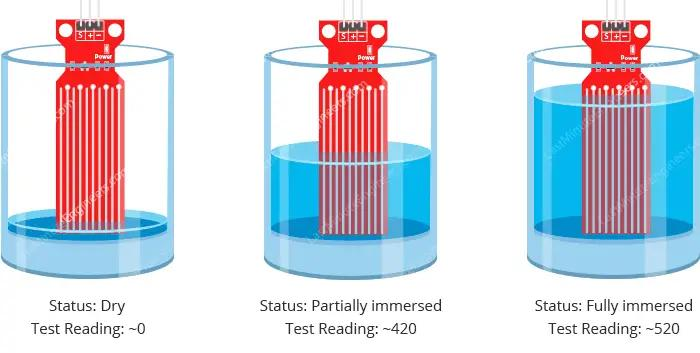
\includegraphics[scale=0.55]{Water-Level-Sensor-Calibration}
		\caption{Sensor response to different water levels.}
		\label{water_level_sensor_basics}
	\end{center}
\end{figure}









\subsection{Circuit}

The circuit for this sensor is fairly simple. All we need to do is provide a ground and power source to make it work, and then a connect a wire from the sense pin on the sensor to an analog pin on the Arduino.



\begin{figure}[H]
	\begin{center}
		%\title{}
		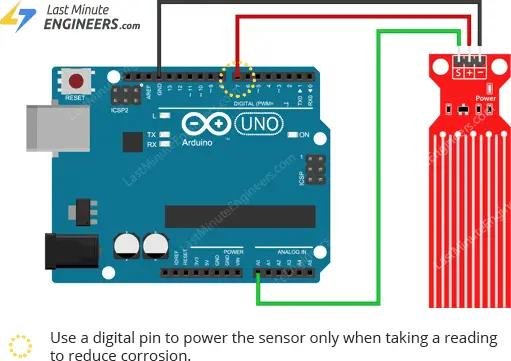
\includegraphics[scale=0.55]{circuit_water_sensor_basic}
		\caption{Sensor response to different water levels.}
		\label{circuit:water_sensor_basic}
	\end{center}
\end{figure}














\subsection{Program}











\subsection{Experiment}

We are going to perform an experiment with this sensor. 


\noindent $\bigcirc$ Objective: Create a chart of the sensors output for a range of different water levels in the cup. You can use Google Spreadsheets to record your results.

\noindent $\bigstar$ Bonus: 








\subsection{If Statements}


\noindent $\bigcirc$ Objective: Add 3 LEDs to your circuit: a green, yellow and red one. Make the LEDs turn on only when:
\begin{enumerate}
	\itemsep -1em
	\item Green - the cup is $1/4$ full or more
	\item Yellow - the cup is $1/2$ full or more
	\item Red - the cup is $3/4$ full or more
\end{enumerate}

\noindent Use pins 9, 10 and 11 to control your 3 LEDs.

\noindent $\bigstar$ Bonus (A big challenge!): Can you make the LEDs progressively light over their ranges? You will need to use the map function and PWM output to make this work. For example, the yellow LED should remain fully off until the green LED is at full brightness when the cup is $1/4$ full. Then, as the cup fills up from $1/4 \rightarrow 1/2$, the yellow LED should progressively get brighter and brighter.

\begin{enumerate}
	\item 
\end{enumerate}




















\section{Ultra-Sonic Range Finder}

\subsection{How it works}

The ultrasonic sensor is capable of measuring distances between 2 cm and 400 cm (4 meters). It does this by emitting a short sound wave and listening for an echo. The duration of time between the initial sound pulse and the echo can be used to determine how far away the object is.

\subsection{Circuit}

\subsection{Program}

\subsection{Experiment}







\section{Line Detector}

\subsection{How it works}

\subsection{Circuit}

\subsection{Program}

\subsection{Experiment}




\newpage
%\bibliographystyle{numeric}
%\bibliography{bibliography}

\printbibliography


%\begin{thebibliography}{1}
	
%	\bibitem{LME water sensor} https://lastminuteengineers.com/water-level-sensor-arduino-tutorial/

%\end{thebibliography}

\end{document}




 




%Outline for function calls

%\begin{figure}[H]
%\begin{center}
%\title{}
%\includegraphics[scale=0.7]{HallEffect}
%\caption{Diagram showing current flow and build up of charge due to electric and magnetic %fields.\cite{Fitzpatrick}}
%\label{fig:pic}
%\end{center}
%\end{figure}

%\begin{equation} \label{eq:Lorentz}
%\vec{F}=q(\vec{E}+\vec{v} \times \vec{B})
%\end{equation}

%\cite{memoir}
%\ref{eq:Lorentz}

%\bibitem{memoir} Bridgman, P. W. "Biographical Memoir of Edwin Herbert Hall." BIOGRAPHICAL MEMOIRS (n.d.): 79-82.  \url{http://www.nasonline.org/publications/biographical-memoirs/memoir-pdfs/hall-edwin.pdf}. Web. 11 Apr. 2015.
